\documentclass[a4paper, 11pt]{article}

\usepackage{amsmath}
\usepackage{amssymb}
\usepackage{amsthm}
\usepackage{url}
\usepackage{graphicx}
\usepackage{hyperref}

% Theorem Styles
\newtheorem{theorem}{Theorem}[section]
\newtheorem{lemma}[theorem]{Lemma}
\newtheorem{proposition}[theorem]{Proposition}
\newtheorem{corollary}[theorem]{Corollary}
% Definition Styles
\theoremstyle{definition}
\newtheorem{definition}{Definition}[section]
\newtheorem{example}{Example}[section]
\theoremstyle{remark}
\newtheorem{remark}{Remark}

\begin{document}

\title{A predictive model for the Crowds protocol}
\date{\today}
\author{Marco Tinacci}
\maketitle

All the material of this work, included this document, can be found in the public repository \url{https://github.com/marcotinacci/predictive-crowds}.

\section{Introduction} % (fold)
\label{sec:introduction}
In this work we deal with the anonymity protocol CROWDS~\cite{DBLP:journals/tissec/ReiterR98}, we formulate the problem in three different ways extending the canonical set of rules with the possibility to give some inputs to tune the protocol's behavior. In Section~\ref{sec:preliminaries} we will introduce the protocol and the preliminary concepts that we are going to use, in Section~\ref{sec:models} we describe the three models and we show the respective achieved results and finally in Section~\ref{sec:future_work} we conclude discussing possible evolution of the work.
% section introduction (end)

\section{Preliminaries} % (fold)
\label{sec:preliminaries}

\subsection{CROWDS protocol} % (fold)
\label{sub:crowds_protocol}
The crowds protocol has been invented to preserve the anonymity of the sender of a message inside a network of communicating nodes. This approach is useful when corrupted nodes are present in the network and an external attacker may exploit information leaks to trace the origin of the message. For this purpose the protocol intuitively needs to show the sender as the origin of the message not more likely than the other nodes. To do so we use the following randomized algorithm:
\begin{enumerate}
	\item the sender selects a crowd member at random (possibly itself), and forwards the message to it,
	\item the selected router flips a biased coin. With probability $1-p_f$, where $p_f$ (forwarding probability) is given and globally known, it delivers the message directly to the destination. With probability $p_f$, it selects a crowd member at random (possibly itself) as the next router in the path, and forwards the message to it, re-encrypted with the appropriate pairwise key. The next router then repeats this step.
\end{enumerate}
% subsection crowds_protocol (end)

\subsection{Discrete-time Markov chains} % (fold)
\label{sub:discrete_time_markov_chains}

The following definition describe the basic model used in all the three models analyzed in this work.

\begin{definition}\label{def:dtmc}
A discrete-time Markov chain (DTMC) $\mathcal{D}$ is defined as follows
$$ \mathcal{D} = \langle S, \pi, T \rangle $$
where
\begin{itemize}
	\item $S$ is a finite set of states,
	\item $\pi \in \Delta(S)$ is the initial distribution over states,
	\item $T: S \rightarrow \Delta(S)$ is the transition function.
\end{itemize}
\end{definition}

We denote the number of states $|S|$ as $n$. A DTMC $\mathcal{D}$ describe an stochastic dynamic system whose dynamics can be summarized with a stochastic matrix $A \in [0,1]^{n \times n}$. We can estimate future states of the system by multiplying the current distribution, a Dirac distribution pointing to the current state, by $A$ many times, one for every step forward. If we denote the current distribution $x_0 \in [0,1]^n$ we can describe the canonical dynamic of a DTMC with the following equation:
$$ x(k+1) = A \cdot x(k) $$
Using this rule we are able to predict how the probability mass is going to spread after a number of discrete steps $T \in \mathbb{N}$, indeed this measure, also known as transient probability, can be computed in the following way
$$ x(T) = A^T \cdot x_0 $$
The common target of the three models we considered is to tune the dynamics of the DTMC with some input that can affect state probabilities, edge probabilities or probability flow in order to obtain a transient probability that will preserve the anonymity of the sender.
% subsection discrete_time_markov_chains (end)
% section preliminaries (end)

\section{Models} % (fold)
\label{sec:models}

% section models (end)

\subsection{Input control array} \label{subs:inputcontrol}

\paragraph{Probabilistic behavior}
We model the protocol as a DTMC, states represent nodes of the network and edges represent transitions of the message from a node to another. Message forwarding is a probabilistic choice among nodes of the network. We can describe the dynamics of the protocol by using a stochastic matrix $A \in \mathbb{R}^{n\times n}$, with $n$ the number of nodes of the network. Since $A$ is stochastic the following condition holds

\begin{equation} \label{eq:stoc1}
a_{ij} \in [0,1],\ \forall i,j = 1,\dots,n
\end{equation}
\begin{equation} \label{eq:stoc2}
\sum_{i=1}^n a_{ij} = 1,\ \forall j = 1,\dots,n
\end{equation}

Let $a_{ij}$ be an element of $A$, we can describe how the dynamics modify the state using the following system

\begin{equation} \label{eq:system}
	x_j(k+1) = \sum_{i=1}^n a_{ij} x_i(k), \ \forall j = 1,\dots,n
\end{equation}

where the state $x(k) \in \mathbb{R}^n$ with $k \geq 0$ represents a probability distribution over states, then it holds $\sum_{i=1}^n x_i(k) = 1$ and $x_i(k) \in [0,1]$ for any $i = 1,\dots,n$.

\paragraph{Predictive control} % (fold)
\label{par:predictive_control}
We introduce a vector of parameters $u(k) \in \mathbb{R}^n$ at time $k$ that affect the system dynamics in the following way

\begin{equation} \label{eq:mpc}
		x(k+1) = Ax(k) + Bu(k)
\end{equation}

% TODO correggere dimensione B
for $k \in \mathbb{N}_0$ and $B \in \mathbb{R}^{n\times n}$. $B$ is a constant real square matrix that describe how parameters affect the state evolution.

% paragraph predictive_control (end)

\paragraph{Constraints} % (fold)
\label{par:constraints}
To preserve the probability distribution structure of the state we must ensure that, given any correct $x(k)$, the respective evolution $x(k+1)$ is still correct, that is $x(k+1) \in [0,1]^n$ and $\sum_{i=1}^n x_i(k+1) = 1$. From the former condition we derive the following constraints

\begin{equation} \label{eq:constr1}
	-1 \leq -\sum_j^n a_{ij} x_j(k) \leq \sum_j^m b_{ij} u_j(k) \leq 1 - \sum_j^n a_{ij} x_j \leq 1
\end{equation}
while, from the latter, we can derive
\begin{equation} \label{eq:constr2}
	\sum_{i=1}^n\sum_{j=1}^m b_{ij} u_j(k) = 0
\end{equation}


% paragraph constraints (end)

\paragraph{Objective} % (fold)
\label{par:objective1}
We use the canonical performance index (\ref{eq:performanceindex1}) for quadratic programming and we customize values in $P,Q \in \mathbb{R}^{n\times n}$ and $R \in \mathbb{R}^{m\times m}$ matrices to suit our target.
\begin{equation} \label{eq:performanceindex1}
	J(x(0),U) = x(N)^T P x(N) + \sum_{k=0}^{N-1} x(k)^T R x(k) + u(k)^T Q u(k)
\end{equation}
We are interested in maximizing the probability of being in a healthy node, with a priority for the receiver, and in minimizing the probability of using a corrupted node. 
% paragraph objective (end)

\paragraph{Results} % (fold)
\label{par:results}

We developed a MATLAB script that implement the crowds scenario we defined in this section. We used YALMIP~\cite{YALMIP} to formulate the problem, generalizing it on the dimension of the network, on the number of corrupted nodes, on the number of parameters employed, on the length of the horizon and on the forward probability. In Figure~\ref{fig:mpc} the predicted state behavior is represented (above) with the respective control actions (below) over time. We can see that healthy nodes (in blue) will be reached with a higher probability with respect to corrupted nodes (in red). The receiver (in green) has the highest probability due to the relatively high forward probability $p_f$. If we increase the number of control inputs, that in this test is $3$, the blu lines tend to move away from the red lines, still remaining close to each other, while red lines tend to move close to zero.

\begin{figure}[htbp]
	\begin{center}
	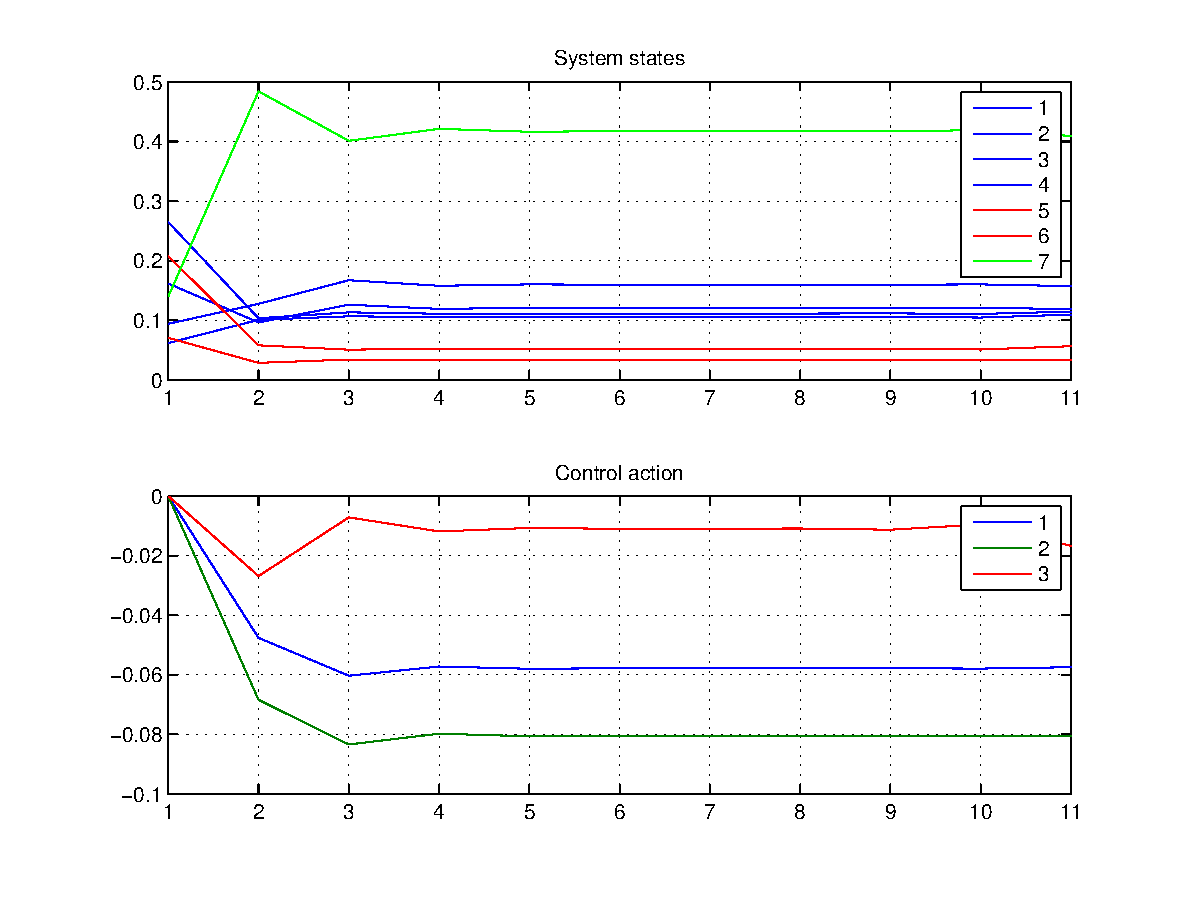
\includegraphics[width=.8\textwidth]{images/mpc}
	\end{center}
	\caption{Control of a crowds network of 7 nodes with 3 parameters with model predictive control}
	\label{fig:mpc}
\end{figure}

The results represented in Figure~\ref{fig:mpc} derive from an experiment with the following settings: 
\begin{itemize}
	\item the network contains $4$ healthy nodes, $2$ corrupted nodes and $1$ receiver;
	\item the prediction horizon is $10$;
	\item $3$ input parameters are used.
\end{itemize}
To maximize the probability of using a healthy node instead of a corrupted one we set weights in the performance index (\ref{eq:performanceindex1}) in the following way
\begin{equation} \label{eq:pqmatrix}
	P = Q = 10 \cdot I
\end{equation}
\begin{equation} \label{eq:rmatrix}
	r_{ij} = 
	\begin{cases}
		1 & \mbox{if } i=j \mbox{ and $i$ is a healthy node} \\
		10 & \mbox{if } i=j \mbox{ and $i$ is a corrupted node} \\
		0 & \mbox{if } i\neq j \\
	\end{cases}
\end{equation}
where $r_{ij}$ is an element of $R$. The MATLAB code used to run this experiment can be found in the github repository \url{https://github.com/marcotinacci/predictive-crowds/blob/master/mpc_crowds_yalmip.m}.
% paragraph results (end)

\subsection{Input control matrix}
We consider a variation of the control applied in the first model from Section~\ref{subs:inputcontrol}, since every input parameter may affect more than one transition probability and, on the other side, every probability could be affected by more than one input parameter. This kind of formulation does not make clear what control input actually are in the concrete scenario, thus we reformulate the problem in order to have a one-to-one relation between control inputs and transition probabilities. We consider the same stochastic matrix $A$ and constraints (\ref{eq:stoc1}) and (\ref{eq:stoc2}) to represent the system dynamics, but we change the control parameters in order to act on the specific transition probabilities.

\paragraph{Predictive control}
We introduce the possibility to tune probabilities over the edges of the DTMC preserving the distribution constraints (\ref{eq:stoc1}) and (\ref{eq:stoc2}). Let $U \in \mathbb{R}^{n\times n}$ be the input matrix that will be used to tune the probabilities. In order to preserve the distribution constraints of $x(k)$ the following condition must hold on $U$
\begin{equation} \label{eq:zerosum}
	\sum_{j=1}^n u_{ij}(k) = 0
\end{equation}
where $u_{ij}(k)$ is an element of $U(k)$ and $k \geq 0$, for any $i = 1,\dots,n$.

Now we can extend the system dynamics (\ref{eq:system}) with parameters given by $U$ in this way
\begin{equation} \label{eq:system_extended}
	x_j(k+1) = \sum_{i=1}^n a_{ij} x_i(k) + u_{ij}(k), \ \forall j = 1,\dots,n
\end{equation}
It is easy to see that, if (\ref{eq:zerosum}) holds and $x(k)$ is a valid distribution, $x(k+1)$ is a distribution as well.

\paragraph{Constraints}
Since parameters $U(k)$ can increase or decrease transition probabilities $A$ out of the probability range $[0,1]$ we need to fix individual constraints to avoid that. Parameter $u_{ij}(k)$ is a local absolute modification of the probability mass flowing in a specific edge at time $k$, thus, starting from $a_{ij}x_j(k)+u_{ij}(k) \in [0,1]$ we can derive the following constraints

\begin{equation} \label{eq:constraints}
	-1 \leq -a_{ij}x_j(k) \leq u_{ij}(k) \leq 1-a_{ij}x_{j}(k) \leq 1
\end{equation}

\paragraph{Objective} % (fold)
\label{par:objective2}
We define a performance index with two features: firstly, minimizing the euclidean distance between the current state $x(k)$ and the ideal state $x_{id} \in [0,1]^n$, that is the distribution we want to obtain from the system; secondly, penalizing high modifications of input controls with specific costs. We use a weight vector $w^x$ to realize the former feature, while we use a weight matrix $W^u$ for the latter, to measure the effort of every input control on every probabilistic transition. The performance index is defined as follow
\begin{equation} \label{eq:index_ext}
	J(x(0),U) = \sum_{k=0}^{N-1}\sum_{i=1}^{n}\sum_{j=1}^{n} w_i^x(x_i(k) - x_{id})^2 + w_{ij}^u u^2_{ij}(k)
\end{equation}

Thus the problem can be summarize as the following optimization

\begin{equation} \label{eq:opt2}
	\begin{array}{ll}
		\underset{U}{\mbox{min}} & J(x(0),U) \\
		\mbox{subject to} &
		(\ref{eq:zerosum})(\ref{eq:system_extended})
		(\ref{eq:constraints}) \\
	\end{array}
\end{equation}


% paragraph objective (end)
\paragraph{Results} % (fold)
\label{par:results2}
Again we used the same environment (MATLAB + YALMIP) to formulate the problem and to solve it with quadratic programming. The result is shown in Figure~\ref{fig:qp-states} using the same notation from Figure~\ref{fig:mpc}. The outcome is clearly more accurate than the previous experiment as expected, since we are using more parameters. To be specific we parametrize weights on edges instead of states. Moreover, we do not give a limit to the number of parameters that can be used. In Figure~\ref{fig:qp-params} are shown the parameters affecting the transition probabilities starting from the first state. 

Since the formulation of the problem is different, so it is the parameters setting. In this case we have to chose values for $w^x$, $w^u$ and $x_{id}$, while the rest of the values are the same as the previous experiment. The MATLAB source code to generate this experiment can be found at \url{https://github.com/marcotinacci/predictive-crowds/blob/master/crowds_qp_yalmip.m}.

\begin{equation}
	\begin{array}{l}
		x_{id} = (0.05, 0.05, 0.05, 0.05, 0, 0, 0.8) \\
		w^x = (1, 1, 1, 1, 1, 1, 1) \\
		w^u = \mbox{rand}(N) \\
%		\begin{pmatrix}
%			0.1 & \cdots & 0.1 \\
%			\vdots & \ddots & \vdots \\
%			0.1 & \cdots & 0.1 \\
%		\end{pmatrix} \\
	\end{array}
\end{equation}

We randomized $w^u$ with values in $[0,1]$ in order to distinguish values of the parameters like in Figure~\ref{fig:qp-params} that, in case of uniform costs, would assumed the same value as consequence of (\ref{eq:opt2}).

\begin{figure}[htbp!]
	\begin{center}
	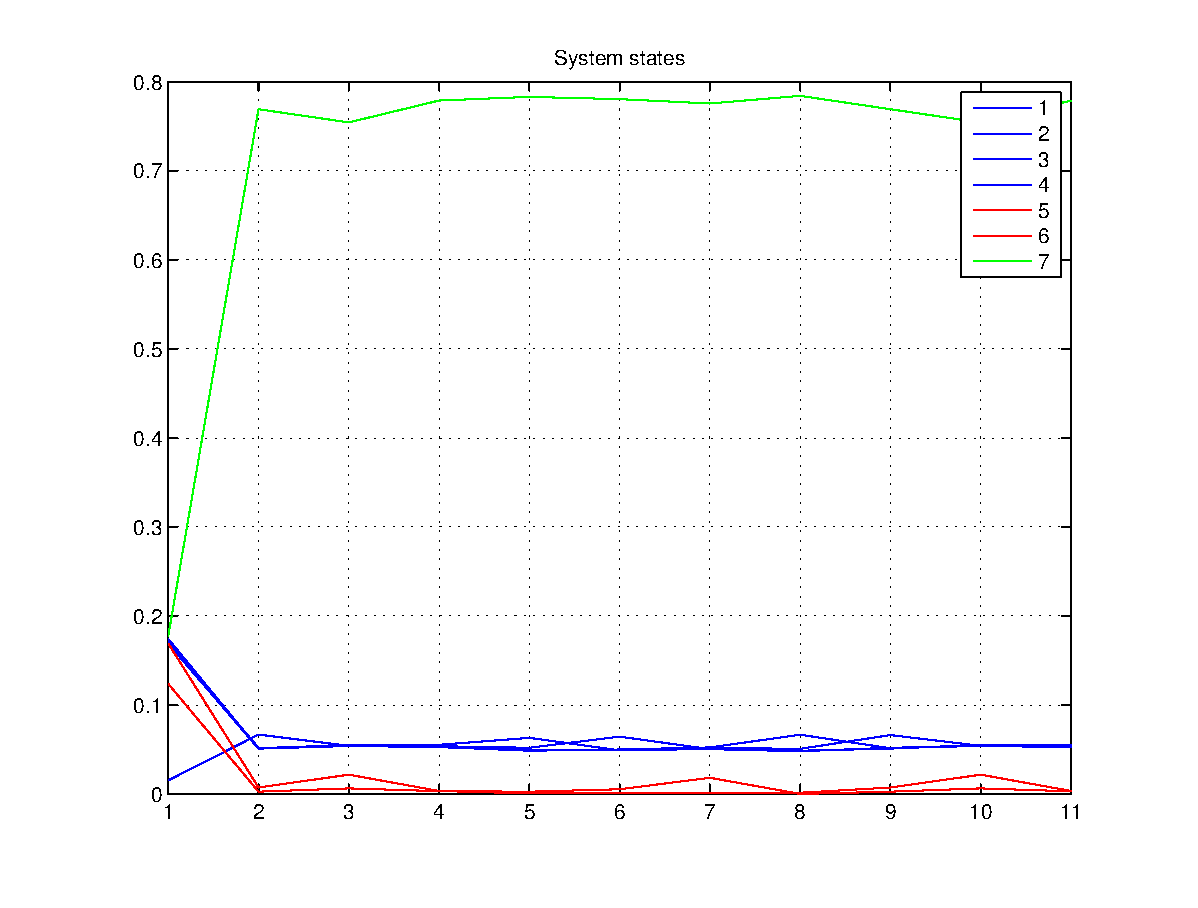
\includegraphics[width=.8\textwidth]{images/qp-states}
	\end{center}
	\caption{Control of a crowds network of 7 nodes with quadratic programming}
	\label{fig:qp-states}
\end{figure}

\begin{figure}[htbp!]
	\begin{center}
	\includegraphics[width=.8\textwidth]{images/qp-params}
	\end{center}
	\caption{Parameter values on edges starting from the first state with quadratic programming}
	\label{fig:qp-params}
\end{figure}

\subsection{Topological control matrix} % (fold)
\label{sub:topological_control_matrix}

We formulate the same problem a third time. In this case we want to tune the weights over transitions before the probability mass is affected by them, like in the work of Bartocci et al.~\cite{DBLP:conf/tacas/2011}. To do so we formulate the problem as follows

\begin{equation}\label{eq:top-system}
	x(k+1) = (A+U(k)) x(k)
\end{equation}

Again, we have the following straightforward constraints:
\begin{itemize}
	\item $A$ is a stochastic matrix,
	\item $x(k)$ is a discrete probability distribution $\forall k=1\dots H$, where $H$ is the chosen horizon,
	\item $U$ is the input matrix that must be zero-sum per columns.
\end{itemize}

The performance index is again (\ref{eq:index_ext}). Using MATLAB and YALMIP we implemented the just described problem (\url{https://github.com/marcotinacci/predictive-crowds/blob/master/crowds_nlp_yalmip.m}). A nonlinear programming solver was used until the last iteration over 1000 cycles, but the results were quite accurate, as shown in Figure~\ref{fig:nlp-states} and Figure~\ref{fig:nlp-params}.

\begin{figure}[htbp!]
	\begin{center}
	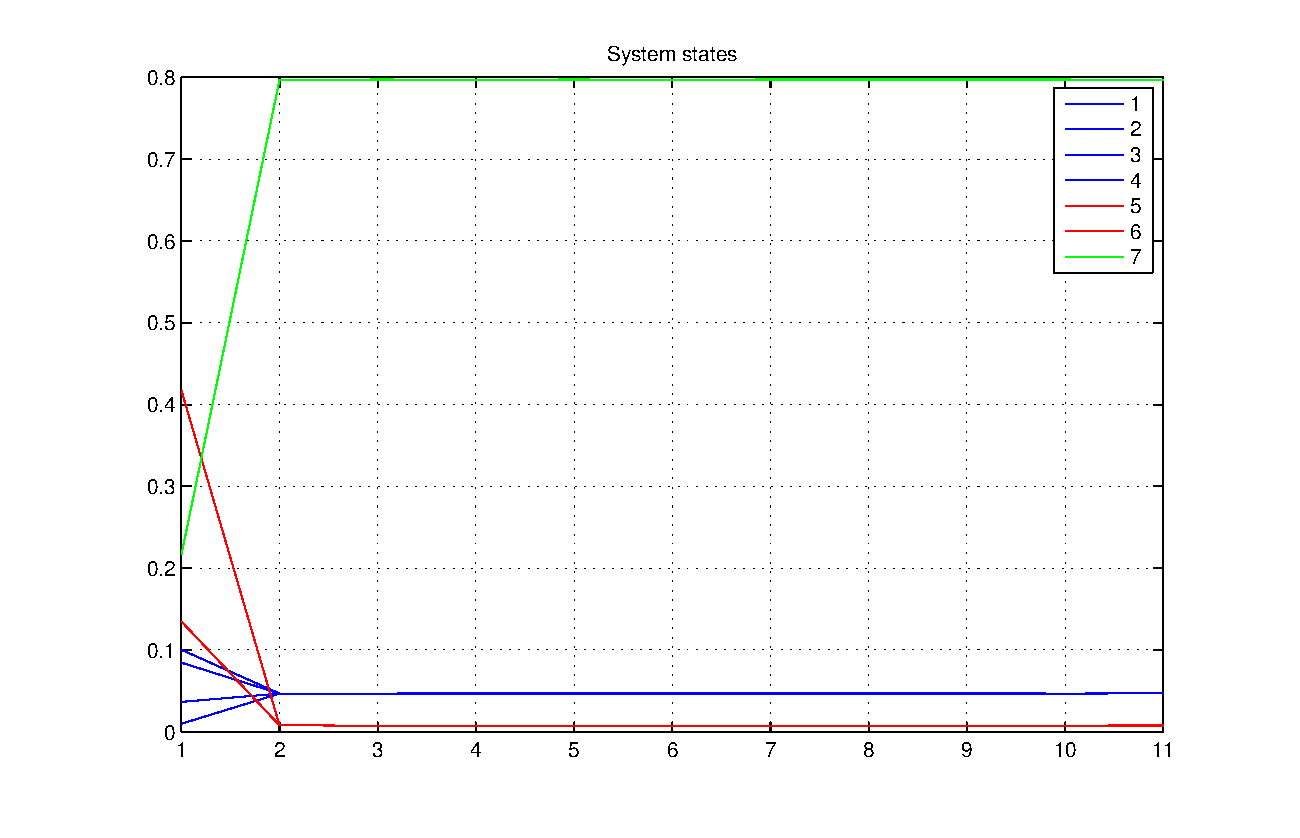
\includegraphics[width=.8\textwidth]{images/nlp-states}
	\end{center}
	\caption{Control of a crowds network of 7 nodes with nonlinear programming}
	\label{fig:nlp-states}
\end{figure}

\begin{figure}[htbp!]
	\begin{center}
	\includegraphics[width=.8\textwidth]{images/nlp-params}
	\end{center}
	\caption{Parameter values on edges starting from the first state with nonlinear programming}
	\label{fig:nlp-params}
\end{figure}

% subsection topological_control_matrix (end)

% paragraph results (end)
\section{Future work} % (fold)
\label{sec:future_work}

At the moment the scenario is not very realistic because we need to know which are the corrupted nodes before, but in that case any path avoiding those corrupted nodes would be a good solution. We could use the concept of partially observable model, like hidden Markov models, to model the perception of a leak of information. In this way penalties given to suspected corrupted nodes may be updated according to the perceived observations. Once the system has been modeled as a hidden Markov model, it can be converted into a DTMC and analyzed as we currently do. This kind of transformation is linear in the number of nodes times the number of observations.

In this work only the classical definition of the crowds protocol has been taken into account and the network is assumed to be strongly connected. Sparsity properties of different kind of topologies, block diagonal or band matrix structures for instance, may be exploited to improve analysis performance.
% section future_work (end)

\bibliographystyle{plain}
\bibliography{biblio}
% TODO repository github

\end{document}
